        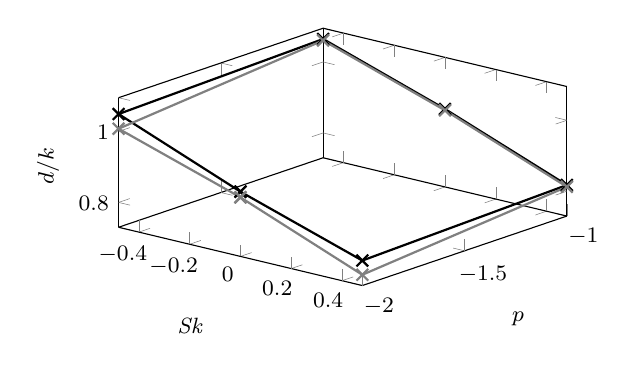
\begin{tikzpicture}[]
        \centering
        \begin{axis}[
        view={40}{35},
            ylabel={$p$},
            xlabel={\textit{Sk}},
			zlabel={$d/k$},
		%	ztick={5.5,6,6.5,7,7.5},
            %zmin=0.06,% ymax=1,
            width=.6\textwidth,
            height=.4\textwidth,
            label style={font=\footnotesize},
            tick label style={font=\footnotesize}
            ]

                        \addplot3 [
            black,mark=x,thick, mark size=3pt
            ]
            coordinates{
            (0,-2,45.62/50)			
			(0.48,-2,40.02/50)
			(0.48,-1,40.87/50)
			(0,-1,47.47/50)
			(-0.48,-1,53.23/50)
			(-0.48,-2,52.45/50)
            (0,-2,45.62/50)
			};
			\addplot3 [
            gray,mark=x,thick, mark size=3pt
            ]
            coordinates{
            
            (0,-2,44.82/50)
			(0.48,-2,38.02/50)
			(0.48,-1,40.62/50)
			(0,-1,47.29/50)
			(-0.48,-1,53.03/50)
			(-0.48,-2,50.38/50)
			(0,-2,44.82/50)
            };
            
                                                %\addplot3 [
            %red,mark=o,thick, mark size=3pt
            %]
            %coordinates{
            %(0,-2,1.58018*0.02+0.061)			
			%(0.48,-2,1.6769*0.02+0.046)
			%(0.48,-1,1.67396*0.02+0.046)
			%(0,-1,1.57652*0.02+0.061)
			%(-0.48,-1,1.45811*0.02+0.074)
			%(-0.48,-2,1.45994*0.02+0.074)
            %(0,-2,1.58018*0.02+0.061)
			%};
			%\addplot3 [
            %%red,mark=o,dotted,thick, mark size=3pt
            %]
            %coordinates{
            
        %    (0,-2,1.51138*0.02+0.061)
	%		(0.48,-2,1.6007*0.02+0.046)
	%		(0.48,-1,1.68346*0.02+0.046)
	%		(0,-1,1.58295*0.02+0.061)
	%		(-0.48,-1,1.46401*0.02+0.074)
	%		(-0.48,-2,1.41258*0.02+0.074)
	%		(0,-2,1.51138*0.02+0.061)
     %       };
        \end{axis}
        \end{tikzpicture}